\documentclass[11pt]{article}
\usepackage[a4paper,margin=1in]{geometry}
\usepackage{amsmath,amssymb}
\usepackage{graphicx}
\usepackage{enumitem}
\usepackage{tikz}
\usetikzlibrary{positioning}
\usepackage{fancyhdr}
\usepackage{tabularx}
\usepackage{array}
\usepackage{xcolor}
\usepackage{titlesec}
\usepackage{lastpage}

\pagestyle{fancy}
\fancyhf{}
\lhead{2501-PYL1003 (Mechanics \& STR) --- Practice Paper 1}
\rhead{Page \thepage\ of \pageref{LastPage}}
\renewcommand{\headrulewidth}{0.4pt}

\titleformat{\section}{\normalfont\bfseries\large}{\thesection.}{0.6em}{}

% Boxed option letter, mimicking the original paper's style
\newcommand{\opt}[2]{%
  \begin{minipage}[t]{0.9\linewidth}
    \fbox{\textbf{#1}}\hspace{0.5em}#2
  \end{minipage}\par\vspace{2pt}
}

\newcounter{qcounter}

\begin{document}

\begin{center}
  {\small\textit{Dept of Physics, IIT Delhi}}
\end{center}

\noindent
\begin{minipage}{0.62\linewidth}
  {\large\bfseries Practice Midsem Examination --- Paper 1}\\[2pt]
  \textit{Based on: 2501-PYL1003 (Mechanics \& STR)}
\end{minipage}
\hfill
\begin{minipage}{0.36\linewidth}\raggedleft
  2501-PYL1003 (Mechanics \& STR)\\
  Course Instructor: Pradipta Ghosh\\
  \textbf{Full Marks: 47, Set-P1}\\
  Practice Mid-sem exam
\end{minipage}

\vspace{6pt}
\noindent\textbf{Name:} \underline{\hspace{6cm}} \qquad \textbf{Entry Number:} \underline{\hspace{4cm}}

\vspace{10pt}
\noindent\textbf{Please read the following instructions carefully}
\begin{itemize}[leftmargin=1.4em]
  \item Please write your name and entry numbers on the question papers at the given places.
  \item An MCQ can also be an MSQ. Explain your answer for the MCQ/MSQ.
  \item Please show the intermediate steps and reasoning for your answers.
  \item Rough work should be shown in the question paper itself.
  \item Approximation, truncation/round-off should be done justifiably.
\end{itemize}

\vspace{8pt}
\hrule
\vspace{10pt}

% ------------------------------------------------------------------
\begin{enumerate}[leftmargin=1.6em, label=\arabic*., itemsep=14pt]

% Q1 --------------------------------------------------------------
\item In terms of the fundamental units (M, L, T, etc.), `power' has the same dimension as \hfill \textbf{2+1 = 3}
\opt{a}{Rate of change of angular momentum}
\opt{b}{Force $\times$ velocity}
\opt{c}{Pressure $\times$ volume $\times$ frequency}
\opt{d}{Impulse $\times$ frequency}

% Q2 --------------------------------------------------------------
\item (i) The dimension of the coefficient of viscosity $\eta$ (defined through $F = \eta A \dfrac{dv}{dx}$, where $F$ is force, $A$ is area, and $\dfrac{dv}{dx}$ is velocity gradient), in terms of the fundamental units (M, L, T, etc.) is \hfill \textbf{1+1+1 = 3}
\opt{a}{$\mathrm{M^1L^{-1}T^{-1}}$}
\opt{b}{$\mathrm{M^1L^{-1}T^{-2}}$}
\opt{c}{$\mathrm{M^{-1}L^1T^{-1}}$}
\opt{d}{$\mathrm{M^1L^{1}T^{-1}}$}

\vspace{4pt}
\noindent (ii) A thin layer of oil of area $2\ \mathrm{m^2}$ is sheared with a velocity gradient of $5\ \mathrm{sec^{-1}}$, producing a force of magnitude $F_0$. Express the coefficient of viscosity $\eta$ of the oil in terms of $F_0$ (write your answer purely in terms of $F_0$ and numbers).

% Q3 --------------------------------------------------------------
\item (i) A drone of mass $0.2$ kg is hovering, then begins to accelerate upward in a straight line from rest, with an acceleration given by $1.2\,t^{n}\ \mathrm{m/sec^2}$, where $t$ is measured in seconds from the instant it starts accelerating. [Neglect air resistance and treat the instant of starting the acceleration as the reference instant, i.e. ignore the effect of gravity on this net acceleration.] Dimensional consistency requires that the value of $n$ is \hfill \textbf{1+1+1 = 3}
\opt{a}{0}
\opt{b}{1}
\opt{c}{$-1$}
\opt{d}{2}

\vspace{4pt}
\noindent (ii) The speed of the drone becomes $9.6$ m/sec at a time $t = m$ sec. The value of $m$ is
\opt{a}{2}
\opt{b}{3}
\opt{c}{4}
\opt{d}{6}

% Q4 --------------------------------------------------------------
\item (i) A woman, standing on a frictionless surface, pushes a hockey puck of mass $0.2$ kg with a force of magnitude $6$ N. Later, she pushes a sled of mass $30$ kg with the same force. The ratio of the resultant acceleration of the puck to that of the sled is (neglecting all forms of friction and the effect of gravity) \hfill $1+\tfrac{1}{2}+1+\tfrac{1}{2} = 3$
\opt{a}{150}
\opt{b}{0.15}
\opt{c}{$6.67 \times 10^{-3}$}
\opt{d}{$1.5\times 10^2$}

\vspace{4pt}
\noindent (ii) The magnitude of the acceleration of the sled, in $\mathrm{m/sec^2}$, is
\opt{a}{0.10}
\opt{b}{0.20}
\opt{c}{30}
\opt{d}{6.0}

% Q5 --------------------------------------------------------------
\item The coordinates of a point $Q$, in Cartesian coordinates, are given as $(x = -6,\ y = 8,\ z = 15)$. The coordinates of $Q$ with respect to the cylindrical polar and spherical polar coordinate systems are written as $(\rho, \phi, z)$ and $(r, \theta, \phi)$, respectively. Which of the following statement(s) is(are) correct? [Hint: for spherical polar, $z = r\cos\theta$. Rounded-off to two decimal places.] \hfill \textbf{1+1+1 = 3}
\opt{a}{$\rho = 10,\ r = 17,\ \phi = 126.87^\circ,\ z = 15$}
\opt{b}{$\rho = 10,\ r = 17,\ \phi = 126.87^\circ,\ \theta = 28.07^\circ$}
\opt{c}{$\rho = 10,\ r = 17,\ \phi = 53.13^\circ,\ \theta = 28.07^\circ$}
\opt{d}{$\rho = 10,\ r = 17,\ \phi = 126.87^\circ,\ \theta = 61.93^\circ$}

% Q6 --------------------------------------------------------------
\item A vector $\vec{B}$, in spherical polar coordinates, is written as $\vec{B} = 4\hat{r} - 3\hat{\theta} + 12\hat{\phi}$. Here $\hat{r}, \hat{\theta}, \hat{\phi}$ are unit vectors along the $r,\theta,\phi$ directions, respectively. If $\hat{i}, \hat{j}, \hat{k}$ represent unit vectors along the $x,y,z$ directions in the Cartesian coordinate system, [Hint: $\vec{r} = x\hat{i} + y\hat{j} + z\hat{k}$, $z = r\cos\theta$, and $\hat{u} = \dfrac{\partial \vec{r}/\partial u}{|\partial \vec{r}/\partial u|}$, where $u = r,\theta,\phi$. Rounded-off to two decimal places.] \hfill \textbf{2+1.5$\times$2 = 5}
\begin{enumerate}[label=(\roman*)]
  \item calculate $\hat{i}$ in terms of $\hat{r}, \hat{\theta}, \hat{\phi}$ at a point $r=1,\ \theta = 60^\circ,\ \phi = 90^\circ$,
  \item calculate $(\vec{B}\cdot\hat{i})\hat{i}$ in terms of $\hat{r}, \hat{\theta}, \hat{\phi}$ at a point $r=1,\ \theta = 90^\circ,\ \phi=0^\circ$,
  \item calculate $(\vec{B}\cdot\hat{i})\hat{i}$ in terms of $\hat{r}, \hat{\theta}, \hat{\phi}$ at a point $r=2,\ \theta = 90^\circ,\ \phi = 180^\circ$.
\end{enumerate}

% Q7 --------------------------------------------------------------
\item For a comet orbiting the Sun, the speed at perihelion is found to be five times the speed at aphelion. Calculate the eccentricity ($\epsilon$) of the orbit. [Orbit trajectory is given as $r = p/(1+\epsilon\cos\theta)$, with $p$ being the semi-latus rectum.] \hfill \textbf{5}

% Q8 --------------------------------------------------------------
\item In the pulley system shown below, a force of magnitude $15$ N is needed to maintain the system in equilibrium, i.e., no net acceleration of block $B$. Calculate (i) the mass ($M$) of block $B$, and (ii) the tension ($T$) in the topmost cable connecting pulley number 1 to the ceiling. (iii) Draw the properly scaled free-body diagram. [Ignore the masses of the pulleys and connecting cables. Also ignore air resistance. Take $g = 10\ \mathrm{m/sec^2}$ acting downward.] \hfill \textbf{1.5$\times$2+2 = 5}

\begin{center}
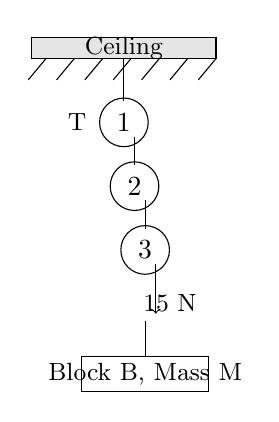
\begin{tikzpicture}[scale=0.9]
  \draw[fill=gray!20] (-1.3,3.6) rectangle (1.3,3.9);
  \foreach \x in {-1.1,-0.7,-0.3,0.1,0.5,0.9,1.3}
    \draw (\x,3.6) -- (\x-0.25,3.3);
  \node at (0,3.75) {\small Ceiling};

  \draw (0,3.6) -- (0,3.0);
  \node[draw,circle,minimum size=0.5cm] (p1) at (0,2.7) {1};
  \node[left=1pt of p1] {\small T};

  \draw (0.15,2.5) -- (0.15,2.1);
  \node[draw,circle,minimum size=0.5cm] (p2) at (0.15,1.8) {2};

  \draw (0.3,1.6) -- (0.3,1.2);
  \node[draw,circle,minimum size=0.5cm] (p3) at (0.3,0.9) {3};

  \draw (0.45,0.7) -- (0.45,0.3);
  \node at (0.65,0.15) {\small 15 N};
  \draw[->] (0.45,0.3) -- (0.45,0.0);

  \draw (-0.6,-0.6) rectangle (1.2,-1.1);
  \node at (0.3,-0.85) {\small Block B, Mass M};
  \draw (0.3,-0.1) -- (0.3,-0.6);
\end{tikzpicture}
\end{center}

% Q9 --------------------------------------------------------------
\item A stone tied to a string of length $0.8$ m is whirled in a horizontal circle at a constant angular speed of $5$ rad/sec. In terms of fundamental units (M, L, T), the dimension of the centripetal acceleration is the same as that of \hfill \textbf{2+1 = 3}
\opt{a}{Angular velocity}
\opt{b}{Linear velocity divided by time}
\opt{c}{Force per unit mass}
\opt{d}{Both (b) and (c)}

% Q10 --------------------------------------------------------------
\item (i) The position of a particle moving along a straight line is given by $x(t) = 2t^3 - 9t^2 + 12t$ (in metres, with $t$ in seconds), starting at $t=0$. The number of times the particle instantaneously comes to rest for $t > 0$ is \hfill \textbf{1+2 = 3}
\opt{a}{0}
\opt{b}{1}
\opt{c}{2}
\opt{d}{3}

\vspace{4pt}
\noindent (ii) Find the time(s) at which the particle is instantaneously at rest, and determine whether the particle is speeding up or slowing down immediately after each such instant. Justify using the sign of the acceleration.

% Q11 --------------------------------------------------------------
\item A particle of mass $m$ moves under a central force such that its path is a circle of radius $R$ passing through the origin, described in plane polar coordinates by $r = 2R\cos\theta$. Using the general expression for radial acceleration in polar coordinates, $a_r = \ddot{r} - r\dot\theta^2$, together with the fact that the angular momentum $L = mr^2\dot\theta$ is conserved, show that the magnitude of the central force varies as $F \propto 1/r^5$. \hfill \textbf{6}

% Q12 --------------------------------------------------------------
\item Two vectors are given as $\vec{P} = 3\hat{i} - 4\hat{j} + 12\hat{k}$ and $\vec{Q} = -2\hat{i} + \hat{j} + 2\hat{k}$. \hfill \textbf{1+1+1 = 3}
\begin{enumerate}[label=(\roman*)]
  \item Calculate the component of $\vec{P}$ along $\vec{Q}$.
  \item Calculate a unit vector perpendicular to both $\vec{P}$ and $\vec{Q}$.
  \item Calculate the angle between $\vec{P}$ and $\vec{Q}$ (rounded off to two decimal places).
\end{enumerate}

% Q13 --------------------------------------------------------------
\item A block of mass $4$ kg rests on a rough horizontal surface with a coefficient of static friction $\mu_s = 0.4$ and coefficient of kinetic friction $\mu_k = 0.3$. A horizontal force $F$ is gradually increased from zero. Take $g = 10\ \mathrm{m/sec^2}$. \hfill \textbf{1+1+1 = 3}
\opt{a}{The block starts moving when $F$ exceeds $12$ N, and once moving, the net force on it (for constant applied $F = 12$ N) is $0$ N}
\opt{b}{The block starts moving when $F$ exceeds $16$ N, and once moving, the net force on it (for constant applied $F = 16$ N) is $4$ N}
\opt{c}{The block starts moving when $F$ exceeds $16$ N, and once moving, the net force on it (for constant applied $F = 16$ N) is $1.6$ N}
\opt{d}{The block starts moving when $F$ exceeds $12$ N, and once moving, the net force on it (for constant applied $F = 12$ N) is $2.4$ N}

% Q14 --------------------------------------------------------------
\item A particle undergoes two successive displacements described in cylindrical polar coordinates: first from $(\rho,\phi,z) = (2,\,0^\circ,\,0)$ to $(2,\,90^\circ,\,3)$ along the surface of the cylinder $\rho = 2$, and then radially outward to $(5,\,90^\circ,\,3)$. \hfill \textbf{2+2 = 4}
\begin{enumerate}[label=(\roman*)]
  \item Express the position vectors of the initial and final points in Cartesian coordinates.
  \item Calculate the magnitude of the net (straight-line) displacement of the particle, rounded off to two decimal places.
\end{enumerate}

% Q15 --------------------------------------------------------------
\item A satellite of mass $500$ kg is to be placed in a circular orbit of radius $r$ around a planet of mass $M$. Starting from Newton's law of gravitation and the requirement of centripetal acceleration, derive an expression for the orbital period $T$ of the satellite in terms of $r$, $M$, and the universal gravitational constant $G$. Hence, state how $T^2$ scales with $r$ (i.e., state Kepler's third law as it follows from your derivation). \hfill \textbf{5}

\end{enumerate}

\vspace{10pt}
\begin{center}
\textit{--- End of Paper 1 ---}
\end{center}

\end{document}
